% =====================================================================
%  SECCIÓN: Anytime benchmarking (metodología de Weise et al., 2014)
%  Resultados REALES sobre las 38 instancias TSPLIB del paquete oficial
%  k-TSP (Pandiri & Singh 2020 / Helsgaun), referencia = valor LKH-3.
%  Requiere junto al .tex: 01_progreso_agregado.png, 02_ecdf_agregado.png,
%  03_ert_vs_meta.png. Añade el \bibitem{weise2014benchmarking} a la bibliografía.
% =====================================================================

\section{Anytime Evaluation of the Heuristics}\label{sec:anytime}

The end-of-run comparison (Tables~\ref{tab:resumen_gap}--\ref{tab:resultados_Q3})
reports a single value per method. However, the greedy cheapest-insertion
baseline, GRASP and the genetic algorithm are \emph{anytime} algorithms: they
keep a feasible incumbent that improves with more computation, so the stopping
point is an arbitrary choice of the experimenter and a single snapshot can hide
which method is preferable under a given budget~\cite{weise2014benchmarking}. To
make the comparison budget-aware and reproducible, we complement the end-of-run
tables with the anytime benchmarking procedure of
Weise~\textit{et~al.}~\cite{weise2014benchmarking}, run on the \emph{same} 38
TSPLIB instances and the same three quartiles of $k$, using the LKH-3 value as the
reference.

\subsection{Machine-independent time and normalized error}
Following~\cite{weise2014benchmarking}, we replace wall-clock time (which depends
on machine, language and load) by a \emph{machine-independent} measure: the number
of \emph{distance evaluations} (DE), i.e.\ accesses to the distance matrix. Every
run emits \emph{log points} $(\mathrm{DE},\,\text{length})$ each time it produces
or updates a solution, recording the full optimization \emph{trajectory} instead
of only its endpoint. Quality is the normalized error
\begin{equation}
F \;=\; \frac{\text{length}}{\text{BKS}} \;-\; 1 ,
\end{equation}
so $F=0$ is the LKH-3 best-known value and, e.g., $F=0.20$ a tour $20\%$ longer.
To aggregate across instances of different size $n$, the DE axis is scaled by
$n^2$, as suggested in~\cite{weise2014benchmarking}. Each stochastic method is run
$10$ times per instance and quartile; DCIH is deterministic (a single run). All
methods share the same budget of $15\,n^2$ distance evaluations.

\subsection{Progress curves, ERT and ECDF}
From the logged trajectories we build three standard views:
\emph{(i)}~\textbf{progress curves}, the median (over runs) best-so-far error $F$
versus the scaled DE (Fig.~\ref{fig:anytime_progress});
\emph{(ii)}~the \textbf{Estimated Running Time} $\mathrm{ERT}(F_t)$, the expected
DE to reach a target error $F_t$, with the restart estimator
$\mathrm{ERT}=(\sum_i \mathrm{DE}_i)/\#\text{successes}$ where failed runs
contribute the full budget (Fig.~\ref{fig:anytime_ert}); and
\emph{(iii)}~the \textbf{Empirical Cumulative Distribution Function}
$\mathrm{ECDF}(F_t)$, the fraction of runs that reached $F_t$ by a given DE
(Fig.~\ref{fig:anytime_ecdf}). As a scalar summary of each curve we use the area
under it (AUC) on the logarithmic DE axis.

\begin{figure}[t]
    \centering
    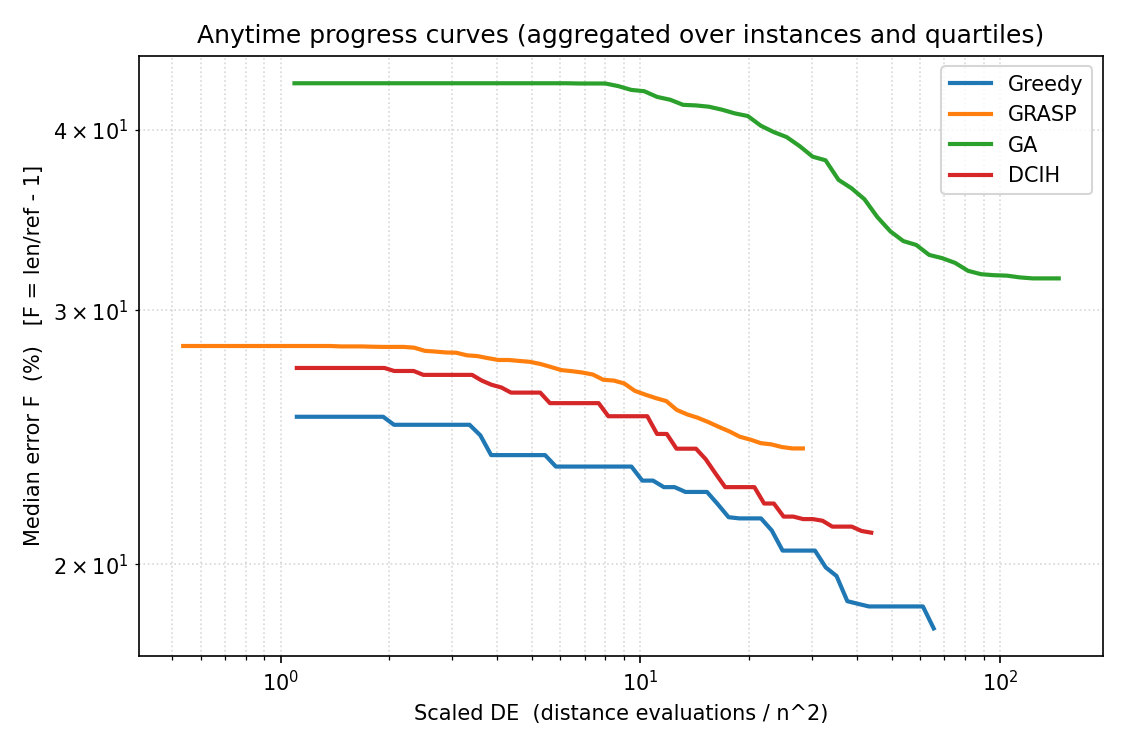
\includegraphics[width=\linewidth]{01_progreso_agregado.png}
    \caption{Anytime \textbf{progress curves} aggregated over the 38 TSPLIB
    instances and the three quartiles of $k$: median best-so-far error $F$ (\%)
    versus the machine-independent time (distance evaluations scaled by $n^2$).
    Lower and earlier is better. The greedy cheapest-insertion baseline dominates
    at every budget, DCIH follows closely and deterministically, and the genetic
    algorithm starts far worse and is still descending at the end of the budget,
    indicating it has not yet converged.}
    \label{fig:anytime_progress}
\end{figure}

\begin{figure}[t]
    \centering
    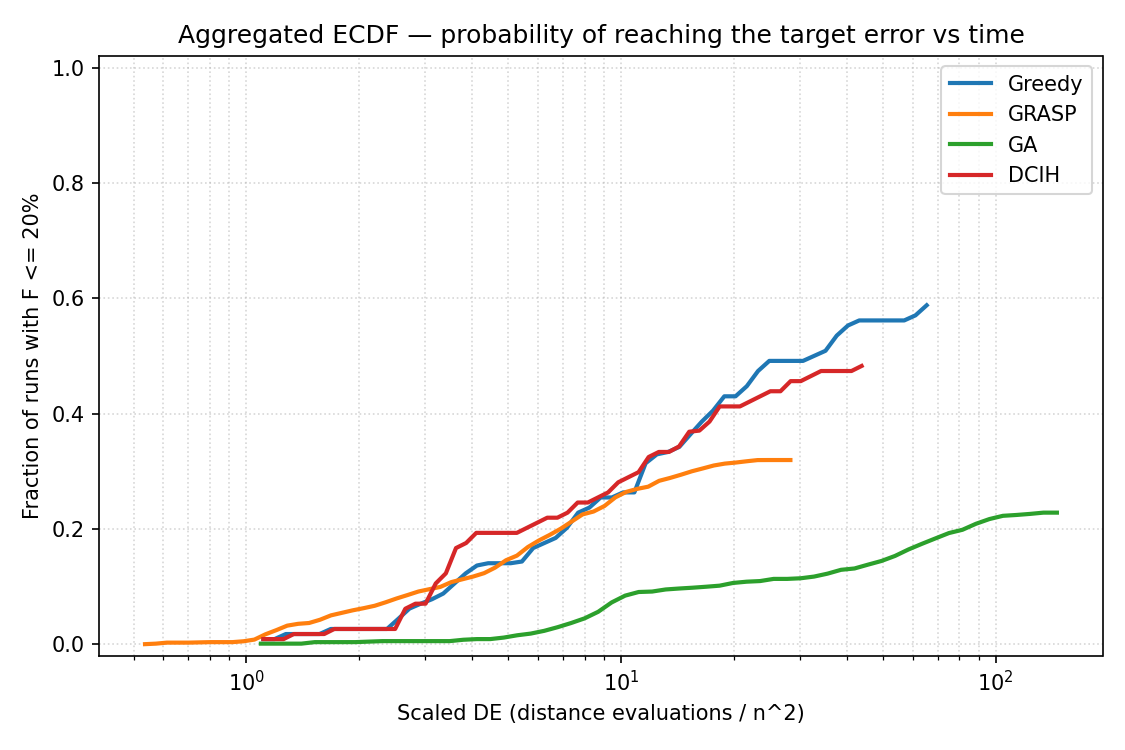
\includegraphics[width=\linewidth]{02_ecdf_agregado.png}
    \caption{Aggregated \textbf{ECDF} for the target error $F_t=20\%$: fraction of
    runs (over instances, quartiles and repetitions) that reach a tour within
    $20\%$ of the LKH-3 reference as a function of the scaled distance evaluations.
    Greedy attains the target in the largest fraction of runs ($\approx59\%$),
    followed by DCIH ($\approx48\%$), GRASP ($\approx32\%$) and GA ($\approx23\%$).}
    \label{fig:anytime_ecdf}
\end{figure}

\begin{figure}[t]
    \centering
    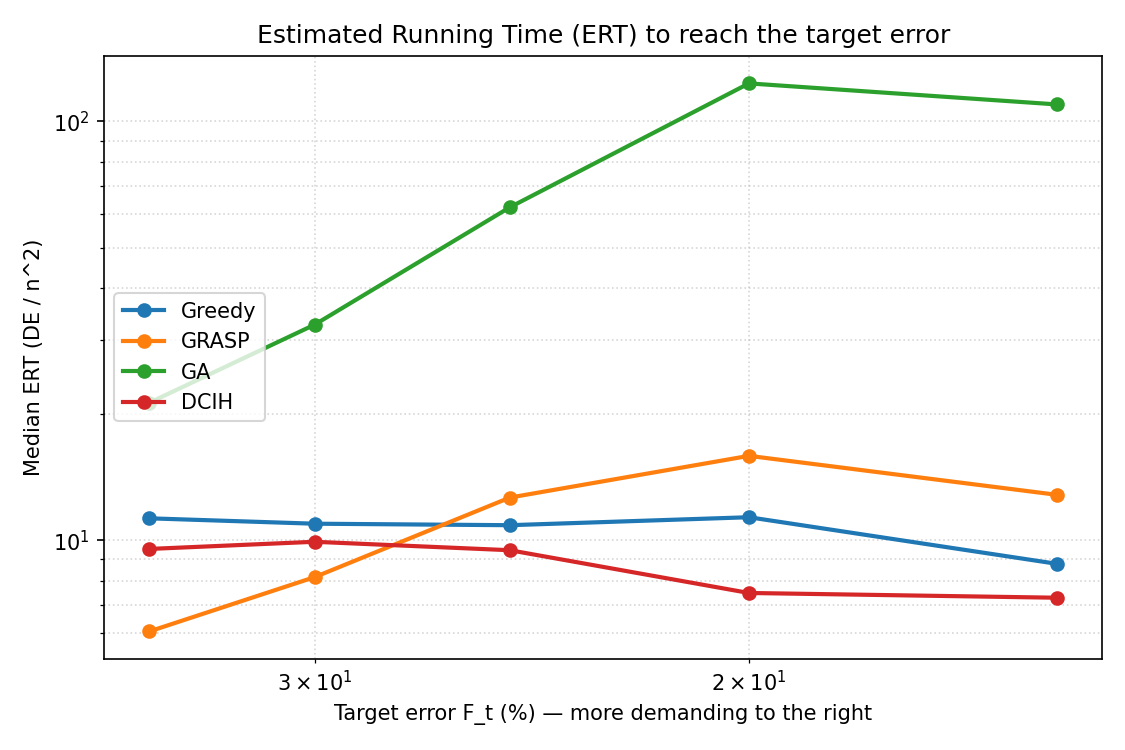
\includegraphics[width=\linewidth]{03_ert_vs_meta.png}
    \caption{Median \textbf{ERT} (scaled distance evaluations, $\mathrm{DE}/n^2$)
    to reach each target error $F_t$ (from $35\%$ down to $15\%$; more demanding to
    the right). Greedy and DCIH reach a given quality with the least computation,
    while the genetic algorithm needs about an order of magnitude more.}
    \label{fig:anytime_ert}
\end{figure}

\subsection{Aggregated ranking}
To condense the views into a single conclusion, on every instance/quartile we rank
the methods by four criteria --- final error, AUC of the progress curve, AUC of the
ECDF, and $\mathrm{ERT}$ at $F_t=20\%$ --- and aggregate by the median rank,
obtaining the global ranking of Table~\ref{tab:anytime_ranking}~\cite{weise2014benchmarking}.
The anytime view is consistent with the end-of-run results
(Tables~\ref{tab:resumen_gap}--\ref{tab:resultados_Q3}): under a fixed
machine-independent budget the greedy cheapest-insertion heuristic is the most
robust method, DCIH provides a competitive \emph{deterministic} trajectory (no
variance across runs), GRASP follows, and the population-based genetic algorithm
converges most slowly and ranks last within this budget. This does not contradict
the advantage of the GA for large $k$: its median error decreases fastest late in
the run (Fig.~\ref{fig:anytime_progress}) and, at the largest quartile Q3, it
approaches the greedy baseline, in agreement with the end-of-run comparison.

\begin{table}[htbp]
\centering
\caption{Anytime \textbf{global ranking} (median rank, lower is better) aggregating
four criteria over the 38 TSPLIB instances and the three quartiles of $k$, with the
LKH-3 value as reference.}
\label{tab:anytime_ranking}
\begin{tabular}{|l|c|c|c|c|c|}
\hline
\textbf{Method} & \textbf{Final} & \textbf{AUC} & \textbf{AUC} & \textbf{ERT} & \textbf{Global} \\
                & \textbf{$F$}   & \textbf{prog.}& \textbf{ECDF}& \textbf{@20\%}& \textbf{rank} \\
\hline
\textbf{Greedy} & 1.5 & 1.0 & 2.5 & 2.50 & \textbf{2.00} \\
DCIH            & 2.0 & 2.0 & 2.5 & 2.50 & 2.25 \\
GRASP           & 3.0 & 3.0 & 2.5 & 2.75 & 2.88 \\
GA              & 4.0 & 4.0 & 3.0 & 3.00 & 3.50 \\
\hline
\end{tabular}
\end{table}

\subsection{Reproducibility}
The procedure is automated in the companion module \texttt{benchmark\_weise}
(Python): it instruments the four methods with the DE counter and log points, reads
the standard TSPLIB instances and the LKH-3 references from the official k-TSP
package, and regenerates every figure and table with a single command. Because the
time axis is machine-independent and the random seeds are fixed, the anytime
results are reproducible across machines.


% ------------------------------------------------------------------
% Añade este \bibitem a tu \begin{thebibliography}:
%
% \bibitem{weise2014benchmarking} T. Weise, R. Chiong, J. L\"assig, K. Tang,
% S. Tsutsui, W. Chen, Z. Michalewicz, and X. Yao,
% ``Benchmarking optimization algorithms: An open source framework for the
% traveling salesman problem,'' \textit{IEEE Computational Intelligence
% Magazine}, vol. 9, no. 3, pp. 40--52, 2014.
% ------------------------------------------------------------------
